%%This is a very basic article template.
%%There is just one section and two subsections.

%%\RequirePackage[latin1]{inputenc}
\documentclass{article}
\usepackage[brazil]{babel}
\usepackage[utf8]{inputenc}
\usepackage{graphicx}
\usepackage{wrapfig}
\usepackage{boxedminipage}
\usepackage{amsmath}
\begin{document}
\bibliographystyle{alpha}
\bibliography{references}

\newcommand{\observednet}{rede social observada} 

\title{NAIF: Network Analysis of Influence Framework}

\section{Introdução}

A análise de redes sociais tem sido utilizada para a investigação
de temas tão diversos quanto a difusão de inovações \cite{Coleman1966},
oportunidades de emprego \cite{Granovetter1995}, prevenção contra fraude
\cite{Neville2005} e marketing \cite{Domingos2001}. Muito dessa pesquisa inicial
se baseia em redes pequenas em torno de indivíduos escolhidos por amostragem
\cite{Wasserman}\cite{Newman2006}, porém a recente disponibilidade de informações
relacionais na internet através de sites de relacionamentos permitiu o
desenvolvimento da análise de redes em larga escala \cite{Boyd2007}. Não
obstante, o meio ainda carece de modelos dinâmicos de representação para redes
sociais observadas a partir do fenômeno digital \cite{Xiang2010} e é justamente
nesse ponto que o trabalho atual se concentra. Nosso objetivo é avaliar as
dificuldades, parâmetros e modelos existentes para a representação e modelagem
não-supervisionada de redes sociais digitais em larga escala e tempo real,
especificamente para aplicações que façam uso da rede para identificar atores
chaves em processos de difusão de conhecimento, inovações e recursos.

\section{Sobre Redes Sociais}

O estudo de rede sociais inicia nas décadas de 40 e 50, inicialmente voltado para
o estudo de pequenos grupos de individuos e suas interações, a rede era mensurada
através de observações, questionários e entrevistas \cite{Wasserman}.
Diferentemente de outras ciências sociais que consideravam apenas os indivíduo e
seus atributos, o estudo das redes sociais considera suas relações e os atributos
dessas relações. A rede social é um fenômeno complexo envolvendo os
relacionamentos de diversos atores em suas particularidades e que, através de um
processo que chamamos de mensuração, pode ser traduzido em uma representação.
Toda representação da rede social, por ser um modelo, é naturalmente parcial e
enviesado. Comumente, as pesquisas de redes sociais trabalham com grafos onde os
vértices são os atores e os arcos entre os vértices são as relações mensuradas; e
matrizes, onde as linhas e colunas são conjuntos de atores e que a posição
$(i,j)$ da matriz representa o arco \textbf{do} ator $i$ \textbf{para} o ator
$j$. Para economizar repetições, no decorrer deste trabalho quando estivermos nos
referindo ao fenômeno observado, utilizaremos o termo \textbf{\observednet},
enquanto que os termos \textbf{representação} e \textbf{rede social} serão
intercambiáveis.

Devido à disponibilidade de ferramentas matemáticas para o tratamento de grafos,
a análise de redes sociais desenvolveu-se rapidamente construindo métodos e
modelos estatísticos apropriados \cite{Butts2009}. A partir desse ferramental, o
ramo das ciências sociais passou a quantificar diversos fenômenos antes
considerados apenas do ponto de vista subjetivo, como a proeminência dos atores,
que estaria relacionada com a sua centralidade no grafo.

\subsection{Alguma Formalização}

Representamos a rede como um grafo $G(V,E)$ onde $V$ é um conjunto de $n$
vértices (também chamados de atores) e $E$ o conjunto de arestas que os conectam.
Quando a representação é não-direcionada o par $(i,j)$ é chamado de aresta e
temos que $(i,j) \in E$ implica $(j,i) \in E$. No caso em que há direcionamento,
essa afirmação não se sustenta e por isso $(i,j) \in E$ não implica em $(j,i) \in
E$ necessariamente, além do que chamamos o par de arco de $i$ para $j$. De
maneira geral, sempre trataremos a representação como sendo direcionada.

Definimos a matriz de adjacência da rede $X$ com $n$ linhas e colunas, onde
$x_{ij} = 1$, se $(i,j) \in V$ ou 0 de outra forma. Essa matriz de $X$ é uma
representação binária da rede. Podemos generalizar essa notação para incluir
redes com valores discretos onde $0 \leq x_{ij} \leq m$ ou contínuos dispostos em
um intervalo. Ambas as notações, de grafo e de matriz, serão usadas de forma
intercalada neste trabalho.

\section{Sobre Proeminência}

Proeminência é a característica dos relacionamentos de um ator que o põe em
evidência para outros atores na rede \cite{Wasserman}. A proeminência,
academicamente, foi separada em dois aspectos: centralidade e prestígio.
Centralidade é como o ator se posiciona na rede, sua interação e envolvimento com
os outros. Prestígio é como os outros atores se posicionam em relação a ele, como
interagem e envolvem-se com ele \cite{Knoke1983}.

Nosso objetivo, identificar atores chaves para processos de influência da rede,
está relacionado diretamente com o conceito de proeminência de forma que podemos
dizer que a usaremos como uma aproximação da influência do ator na transmissão de
conhecimento, inovações e opiniões pela rede. Por estes motivos, cuidado especial
deve ser tomado sobre a forma como calcularemos a proeminência e que
características são esperadas da representação da rede que será mensurada.

Durante décadas pesquisadores de redes sociais se debruçaram sobre o estudo da
proeminência, desenvolvendo inúmeras métricas que conjuntamente são chamadas de
métricas de centralidade. Quando calculadas considerando os caminhos que
\textbf{saem} do ator, referem-se a sua centralidade propriamente dita. Quando
considera-se os caminhos que \textbf{chegam} no ator, referem-se ao seu
prestígio. Não obstante tenha o comum senso de que essas métricas referem-se de
alguma forma à proeminência do ator, a forma específica tem ficado a cargo de
cada pesquisador que já atribuiu ao seu resultado interpretações como autonomia,
controle, risco, influência, corretagem (\textit{brokerage}), independência,
etc.

Freeman revisou as métricas existentes à época \cite{Freeman1979} e as compilou
em três principais centralidades: por grau, por proximidade (\textit{closeness})
e por intermediação (\textit{betweenness}). Interpretando seus resultados em
relação ao quanto o grafo se aproxima de uma estrutura de estrela
(Figura~\ref{fig:star}), sua visão de centralização ideal, onde suas métricas
alcançam o máximo.

\begin{figure}[h!]
  \caption{Gráfico estrela}
  \label{fig:star}
  \centering
    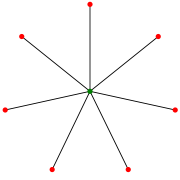
\includegraphics[width=0.3\textwidth]{imgs/star.png}
\end{figure}

Recentemente, Borgatti e Everett \cite{Borgatti2006} nos ofereceram uma
outra reposta para a questão: O que as métricas de centralidade medem? E
chegaram a conclusão que todas elas investigam o relacionamento do nó com os
possíveis caminhos do grafo. Em sua tipologia para a classificação das
métricas de centralidade, propõem quatro dimensões: tipo do caminho,
propriedade do caminho, tipo do envolvimento e forma de agregação. Em outras
palavras, toda métrica de centralidade é uma forma de agregar uma propriedade
dos caminhos de determinado tipo em que o nó tem um determinado envolvimento.
Das quatro dimensões, duas são de maior importância: propriedade do caminho e
tipo de envolvimento. 

\subsection{Tipo de envolvimento} 

O tipo de envolvimento é a dimensão de classificação proposta por Borgatti que
se traduz na maior variância nos resultados. Pode ser de dois tipos: radial ou
medial.

Métricas radiais são as que analisam os caminhos em que o nó está numa das
pontas, ou seja, que saem ou chegam nele. Exemplos de métricas radiais são as
centralidades de grau e proximidade de Freeman. A análise de Borgatti et al veio
confirmar o que as evidências empíricas já sugeriam, que as métricas radiais
representam a parcela de responsabilidade que o nó tem na coesão total da rede e
que, por este motivo, se enfraquecem a medida que a rede não se adequa ao padrão
de núcleo-periferia \cite{Nakao1990}.

Já as ditas mediais analisam os caminhos que passam pelo nó, classificando-o em
seu papel de \textit{gateway} entre partes da rede. O \textit{betweenness} de
Freeman é um exemplo de métrica medial. São mais estáveis em relação à
característica de núcleo-periferia, por outro lado tendem a dar maior importância
a atores que conectam grupos distintos, mas que se encontram na periferia dos
mesmos.

Os dois tipos são complementares e mais de uma métrica devem ser combinadas
(\cite{Stephenson1989}; \textit{Apud} \cite{Wasserman}). Pelo fato de que
usaremos métricas radiais de centralidade para estimar a influência do ator na
rede, já é possível derivarmos uma primeira restrição sobre a representação que
será mensurada:
\paragraph{
\emph{Quanto mais próximo a representação estiver do modelo de núcleo-periferia,
melhor será a aplicabilidade das métricas radiais de centralidade.}}

\subsection{Propriedade do caminho}

Borgatti define dois tipos de propriedade: distância e volume. A
propriedade do tipo distância mais comum é a geodésica que é a quantidade de
arcos presentes no menor caminho entre um ator e outro. Volume refere-se à
quantidade de caminhos entre os nós. As centralidades por grau e
\textit{betweenness} são exemplos de métricas que usam o volume dos caminhos,
enquanto que \textit{closeness} usa distância.

O critério de escolha depende da aplicação. Para o nosso caso, queremos modelar
o efeito da influência entre os pares na transmissão de informação. Nesse
sentido, quanto mais atores próximos estiverem tentando convencer alguém de
algo, maior será sua influência sobre este. Daí temos, naturalmente, a
preferência sobre métricas relacionadas a volume, no lugar de distância, já que
representa diretamente a quantidade de caminhos que existem entre os nós.

\subsection{Métricas de proeminência}

Escolhemos duas medidas para a análise de influência neste trabalho, uma para
centralidade e outra para prestígio. Ambas são do tipo volume, isto é, medem a
quantidade de caminhos, o que representa melhor o fenômeno de pressão social na
difusão de inovações. Para centralidade, utilizaremos a métrica medial
\textit{flow betweenness} que expande o conceito de \textit{betweenness} para
grafos não-binários \cite{Freeman1991} levando em consideração não apenas
geodésicas mas todos os caminhos que passam pelo ator, utilizando o peso das
arestas para medir a ``vazão'' que ``flui'' pelo mesmo. Para prestígio,
escolhemos a métrica radial de poder de Bonacich \cite{Bonacich1987} que
considera a soma dos caminhos que chegam ponderada pelo poder dos atores que a
compõem.

A interpretabilidade de tais métricas está diretamente relacionada com o que está
sendo representado pela rede. É fácil perceber que o poder de Bonacich significa
se o arco do ator $i$ para o ator $j$ quer dizer que $i$ buscou os conselhos de
$j$. 


\cite{Richardson2002} e \cite{Domingos2001}

Durante décadas os pesquisadores de redes sociais se debruçaram sobre o estudo
\begin{wrapfigure}{r}{2in}
\begin{boxedminipage}{2in}
\textbf{\large{Por que etnografia digital não é um bom nome?}}
\normalsize{}

Porque etnografia trata de um estudo aprofundado, qualitativo, do fenômeno
humano. Enquanto que na nossa abordagem digital estamos horizontalizando em
números e mesmo quando verticalizar a abordagem do ponto de vista
``qualitativo'', também será uma abordagem numérica.
\end{boxedminipage}
\end{wrapfigure} da proeminência em redes pessoais, derivadas do círculo
imediato dos atores, por amostragem ou por delimitação teórica. Enfim, vários foram os meios para esse
estudo, mas sempre limitado em quantidade devido ao custo de mensuração da rede.
Esse panorama mudou com a chegada do ciberespaço e as possibilidades de uma
\textbf{etnografia}[buscar termo para inserir aqui] digital. 

\section{redes sociais digitais}

\cite{Clemons2007} sobre redes sociais digitais nao representarem bem a
realidade

Com a era da Internet é fato que pessoas se conectam umas às outras virtualmente
por seu intermédio. A questão é: como mensurar a rede social digital? Definem
sites de redes sociais, um conceito que vamos usar para chegar ao mais amplo,
como sendo um espaço (ciber) em que seja possível 1) criar um perfil, 2)
relacionar uma lista públicade amigos, 3) navegar por essa rede de perfis
interligados. Porém essa definição restringe a sites de relacionamentos
ignorando todo o conteúdo que poderia ser minerado em fóruns e listas de
discussão. Por este motivo, usaremos uma definição mais ampla que chamaremos de
redes sociais digitais como aquelas em que se é possível 1) identificar
unicamente um ator da rede, 2) a interação entre esses atores unicamente
identificados e, em algumas redes mas não em todas, 3) o posicionamento dessa
interação no tempo, permitindo um estudo longitudinal da evolução da rede.

Porque nos parece evidente a impossibilidade aplicar questionários ou
entrevistas com centenas de milhares de atores, respondemos a primeira questão
assim: através de uma etnografia digital, observando as interações dos atores na
rede. A questão que nos aparece agora é como as interações observadas
combinam-se para formar tal rede e se ela é significativa para a aplicação de
técnicas de cálculo de proeminência. A validade dessa observação enquanto
ferramenta prática para mensuração da rede é o tema central deste trabalho.

\section{métricas de proeminência}

Antes de entrar em detalhes sobre como aconteceria essa etnografia digital,
vamos considerar alguns requisitos básicos para as técnicas disponíveis para o
cálculo de proeminência. A literatura sobre proeminência é extensa e propõe
diversas métricas e considerações a serem feitas sobre sua validade. Comum a
todas as técnicas, podemos dizer que duas observações devem ser feitas durante
a escolha do método de pesquisa:
\begin{itemize}
\item Laços de natureza fraca são pouco representativos das escolhas sociais dos
atores. e.g.: estudos mostram que quando questionados, os atores erram em torno
de 50\% a respeito das suas interações com outros atores em comparação com o
observado em campo. Isso se dá devido ao fato que muitas das interações
observadas tem pouca importância relativa para aquelas que o ator se lembra
vividamente.
\item A medição binária, presença ou ausência, da relação não captura a intenção
de escolha dos atores, de forma que não é possível analisar o aspecto de
prestígio dos atores já que não temos informação sobre quem procurou quem.
\end{itemize}

Assim sendo, devemos ser criteriosos na escolha do que observar e de como
combinar as interações observadas de forma a criar uma rede que seja
significativa e direcionada. Esses dois requisitos metodológicos nos guiarão na
concepção de uma etnografia digital voltada a redes sociais.

\section{etnografia digital}

\cite{Spertus2005} - similaridade em orkut


Por etnografia digital entende-se como a etnografia mediada por elementos
digitais. Considerando a produção textual na web, a produção de vídeos dos
respondentes, sua interação com artefatos digitais. Também encontra-se
literatura sobre o uso de artefatos digitais por parte do pesquisador para
registrar e recontar as histórias estudadas. Etnografia, portanto, seria a
atividade humana de observar outros seres humanos e contar sua história. 

Porém, no nosso caso o fenômeno observado é puramente digital. As interações
acontecem na internet. E apesar de entendermos que a rede virtual é uma extensão
que entrelaça a rede física do indivíduo, nosso foco reside totalmente na
virtual. O motivo disso é simples, queremos considerar a maior parte da rede
possível, em toda a sua manifestação, e para isso iremos desenvolver ferramentas
automatizadas que observam e recontam a história da rede de forma apreensível
para nós. Essa observação semi-automatizada é que chamamos de etnografia
digital.

\section{visão etnográfica da rede}

Primeiramente, o pesquisador deve delimitar o fenômeno digital observado. Isso
se dá na escolha dos medianeiros. Chamamos de medianeiros estruturas digitais
(e.g. software) que intermediam a interação humana. Alguns exemplos são: salas
de batepapo, fórums, lista de discussão, sites de relacionamentos, sites de
compartilhamento de fotos e vídeos.

\begin{wrapfigure}{r}{2in}
\begin{boxedminipage}{2in}
No estudo de caso realizado, foi considerada o site de relacionamento Amigos do
C.E.S.A.R. Composto em sua maioria por colaboradores do mesmo, a rede se
configura, portanto, como uma comunidade de prática, i.e. voltada para o
compartilhamento e a colaboração em torno de um foco comum, no caso
desenvolvimento de software. O ambiente foi aberto à pesquisa e por isso podemos
considerar que foi realizada uma análise intrínseca. Todas as informações
utilizadas são também informações públicas na rede.
\end{boxedminipage}
\end{wrapfigure}
Do ponto de vista da análise, podemos considerar duas possibilidades relativas a
um dado fenômeno digital qualquer: a análise intrínseca e a extrínseca. Na
análise intrínseca a observação se dá na própria estrutura digital que media a
interação, por exemplo, a análise tem acesso ao conteúdo e funcionamento
interno (e.g., banco de dados) do medianeiro. Na extrínsica a observação
limita-se ao que está disponível publicamente, sendo restrito o acesso a
conteúdo privativo e comportamental do ator. Questões éticas a parte, não há
dúvidas que o registro da interação do ator \textbf{com} a ferramenta é de
grande valor para o tratamento da atenção como capital social.

\section{a atenção como capital social}

Uma vez que os medianeiros sejam identificados, cabe agora discutir como as
interações observadas serão combinadas para a mensuração da rede. O problema é
que são interações bem diferentes uma das outras e, por isso, com significância
também diferente. Para resolver esse problema iremos considerar a teorial do
capital social que consiste no estudo das transferências de ``recursos'' pela
rede social. A vantagem de utilizar essa teoria é que ela prevê que quanto mais
``recursos'' trafeguem por um laço, mais forte ele é, assim atendendo ao nosso
primeiro requisito para alcançar uma rede com métricas de proeminência
significativas.

Mas que ``recurso'' seria esse que trafega pela rede? Nossa aposta está na
\textbf{atenção}. A atenção é o recurso empregado em cada interação e é o
recurso mais escarço na atual era da informação. Assim como na teoria da
proeminência das redes sociais nós teremos ``estrelas'' e ``isolados'', também
na economia da atenção acharemos esses mesmos atores à medida que mais e mais
atenção eles atraiam sobre si. Para mensurar o quanto de atenção o ator emprega
em sua interação vamos considerar os tipos de interação que ele pode fazer na
rede.

\section{uma tipologia das interações}

Podemos dividir por tipo do conteúdo, abrangência e intenção. Os tipos de
conteúdos podem ser divididos em dois grandes grupos: textuais e não textuais.
Abrangência consiste se a interação é individual básica, individual
desenvolvida, individual generalizado ou comum. Finalmente, quanto a intenção
podemos classificar a interação em assertiva, negativa, conversacional,
informativa, conectiva. É importante ter em mente que as categorias
apresentadas não são, de forma alguma, mutuamente exclusivas, podendo mesmo numa
interação singular ser combinadas em diferentes formas.
\subsection{por conteúdo}
É importante classificar as interações por conteúdo porque cada tipo de conteúdo\begin{wrapfigure}{r}{2in}
\begin{boxedminipage}{2in}
No estudo de caso da rede A.M.I.G.O.S. temos interações que se concentram no
\textbf{texto}: narrativas, comentários, mensagens, fóruns. Temos também
interações \textbf{não textuais}: objetos, avaliações, compartilhamento,
contatos, afiliação a comunidades. No que diz respeito à abrangência, as
interações são do tipo \textbf{indivíduo-generalizada} e \textbf{comum}, dado
que todos os fóruns e narrativas são públicas para toda a rede. Mensagens
privativas não foram analisadas. Não foi realizada uma categorização de
intenção da rede e, por isso mesma, o estudo de caso trata de uma
\textbf{análise ingênua}. Também não foram consideradas \textbf{interações
passivas}.
\end{boxedminipage}
\end{wrapfigure}carrega um valor diferente de atenção. Se quisermos partir para
uma economia da atenção como capital social na rede, precisaremos ser capazes
de medir o grau de atenção dada à interação por parte dos atores envolvidos.
Mais a frente mostraremos nossa abordagem quanto ao tratamento de conteúdos
textuais.
\begin{description}
\item[conteúdo textual] Já foi dito o quanto o texto é importante para a
comunicação mediada por computador, mesmo numa época em que o compartilhamento
de vídeos está na moda, o texto, na forma de comentários, continua sendo o
principal móvel das trocas sociais. São desse tipo:
\begin{itemize}
  \item comentários
  \item mensagens
  \item tópicos
  \item blogs e similares
  \item microblogging e similares
  \item descrições
\end{itemize}
\item[conteúdo não-textual] Nesse grupo estão relacionados não só as interações
áudiovisuais, mas também as interações ``mudas'' como a formação de laços
explícito entre os atores, a classificação uns dos outros através de um
ranqueamento ou simplismente o atestado de ``gostei''/''não gostei'' e o
compartilhamento de conteúdo produzido por um terceiro. Exemplos:
\begin{itemize}
  \item fotos
  \item vídeos
  \item links
  \item laços explícitos entre os atores
  \item rating
  \item compartilhamento
\end{itemize}
\end{description}
\subsection{por abrangência}
A abrangência define quais são os atores influenciados pela interação. Quando um
ator se propõe a investir sua atenção numa interação com a rede, essa proposta
deve ser analisada em vista ao público-alvo da interação. Dessa forma, a
abrangência define o grupo de atores em relação ao qual o ator interagente busca
se posicionar na rede.
\begin{description}
\item[individual básica] Classificam-se neste grupo as interações de caráter
privativo que partem de um ator específico para outro ator. As interações que
tipicamente pertencem a este grupo são as mensagens, os pedidos de conexão e o
compartilhamento de conteúdo do tipo ``forward''.
\item[individual desenvolvida] Quando a interação se inicia em um ator e envolve
sua rede imediata de contatos sem estar publicamente disponível para qualquer
membro da rede. São desse grupo, em sua maioria: tópicos de fóruns, fotos,
vídeos, compartilhamentos, microblogging.
\item[individual generalizada] Quando a interação se inicia em um ator e
torna-se pública para todos os atores da rede. Todos os tipos de interação podem
se classificar nesse grupo, depende do grau de livre acesso que a rede
proporciona aos seus membros.
\item[comum] Quando a interação se dá num espaço de igualdade, quer dizer, que
todos podem interagir com todos no mesmo nível, chamamos de interação comum. Um
exemplo claro dessa categoria é as salas de batepapo onde todos podem publicar
mensagens para todos lerem. Listas de discussão também seguem esse modelo.
Um Blog em particular não é uma interação comum, na maioria dos casos, porque
só o mantenedor do blog pode publicar artigos nesse blog, já o espaço de
comentários do artigo possa ser considerado um espaço comum.
\end{description}
\subsection{por intenção}
Por último, mas não por menos, temos a intenção sobre a qual o ator reveste sua
interação. A diferença de intenção não só pode representar mudança significativa
na quantidade de atenção cedida, como necessariamente define os possíveis
resultados da interação. Podemos classificar a intenção das interações, no
escopo proposto por esse trabalho, em cinco grandes grupos:
\begin{description}
\item[afirmativa] Trata da afirmação de suporte social entre um ator e outro.
Pode ser um comentário positivo relacionado a uma interação prévia do ator
elogiado, uma avaliação positiva, a recomendação do seu conteúdo para outros.
\item[negativa] Quando a interação se dá para depreciar o outro. Pode ser por
comentário, tópicos, mensagens, avaliação negativa.
\item[conversacional] Quando a interação tem caráter pessoal, relacionado a uma
conversação que se inicia ou que está em andamento.
\item[informativo] Quando a intenção é informar um grupo de atores sobre
determinado assunto. Avisos, artigos, propaganda, críticas.
\item[conectivos] Quando a intenção é formar laços explícitos através da rede.
Pedidos para conexão como adicionar à lista de contatos/amigos/etc.
\end{description}
Ainda em relação à categorização das interações por tipo de intenção, temos que
tal realização é cai na área do tratamento de linguagem natural e ainda sem uma
técnica que se compare com a habilidade discriminante do ser humano para a
maioria das interações. Por este motivo, essa categorização é particularmente
complexa do ponto de vista computacional e por isso teremos o cuidado de anotar
as análises de redes sociais digitais que não levem em consideração a intenção
como \textbf{análises ingênuas}.
\subsection{interações passivas}
Para finalizar essa seção sobre interações, falaremos aqui de interações
passivas e comportamentais que podem levar a um maior entendimento de como o
ator investe sua atenção na rede e, por isso mesmo, como se posiciona na rede em
relação a outros atores. Podemos considerar como interação passiva como
aquela que não é necessariamente percebida pelos outros atores além do
interagente, nesse tipo de interação encontram-se todas as interações do
ator como o sistema como: mensagens lidas, não lidas, tempo usado para
cada mensagem, perfis visitados, tempo usado na leitura de outros
conteúdos. Essas informações poderiam ser utilizadas numa análise
intrínseca da rede para a concepção de um modelo mais real do interagente
quanto ao dispêndio da atenção.

\section{mensurando a rede a partir de interações não-textuais}

\cite{Cooper1997} e \cite{Silverstein2000} - artigo doido sobre formas de
encontrar relacao causal entre variaveis, pode ser usado para dizer que tal
influencia causou tal reacao

\cite{Friedman1999} - traz um modelo interessante baseado em probabilidade da
relacao para aprender relacoes entre atributos de atores, baseado em sua
aparicao estatistica no banco de dados, pode ser util usar isso para ajudar na
mensuracao

Agora que podemos definir os medianeiros e classificar as interações sob estudo
em seus tipos, vamos passar à construção da rede social propriamente dita. Em
primeiro lugar, interações não-textuais não são facilmente integráveis, isto é,
em que se assemelha a interação através de uma foto com a afiliação comum a
um mesmo grupo? Por este motivo, a primeira abordagem é separar a rede por
interação, ou seja, cada interação não-textual produz uma rede diferente.
Podemos restringir o total de atenção de cada ator a uma constante, digamos 1
(um), e distribuir sua interação uniformemente sobre o intervalo [0..1].

Essa abordagem será especialmente útil quando formos aplicar a técnica de
medição de proeminência baseada em autovetores mais adiante. Assim, se um
ator escolheu a 5 outros atores para se conectar, cada vínculo terá valor de
0.2. Apesar de incompleta, verificamos que essa abordagem é necessária pois não
tem como conceber um recurso comum, como estabeleceremos mais adiante para as
interações textuais, que trafega pela rede. Como mensurar a atenção
dada/recebida de uma foto? Porém, caso seja possível ao investigador a
utilização de dados sobre a interação passiva dos atores, seria possível
construir uma métrica comum baseada no tempo que o ator gasta observando os
conteúdos alheios.

Mesmo assim, interações como avaliações (ratings) são naturalmente difíceis de
integrar com outras, já que leva a mesma quantidade de tempo para avaliar mal ou
bem o outro ator. Porém, quando levarmos em consideração técnicas como a análise
de sentimentos em texto para a avaliação da intenção das interações, poderemos
imaginar uma integração com avaliações no sentido que elas sao naturalmente
negativas/afirmativas.

\begin{table}[htbp]
	\begin{boxedminipage}{\textwidth}
Para o estudo de caso da rede A.M.I.G.O.S. vamos começar analisando a rede
decorrente das conexões explícitas da rede: os contatos. Contatos são atores
explicitamente adicionados através da ferramenta, constituindo uma interação
não-textual individual-básica. Foram coletadas as interações de 1247 atores
representadas em um digrafo. Desses, 720 formam o componente principal do
digrafo (o maior subgrafo fracamente conexo) e removendo os que se conectam a
apenas 1 indivíduo temos 618 atores e 5180 conexões.
		\large       % tamanho da fonte 
		\setlength{\arrayrulewidth}{2\arrayrulewidth}  % espessura da  linha
		\setlength{\belowcaptionskip}{10pt}  % espaço entre caption e tabela
		\caption{\it Os 10 mais bem posicionados em Proeminência no A.M.I.G.O.S.}
		\centering   % tabela centralizada
		\begin{tabular}{| l | c |}
			\hline
			Ator & Centralidade \\ \hline
			8 & 0.230 \\
			135 & 0.136 \\
			1037 & 0.136 \\
			541 & 0.132 \\
			3 & 0.119 \\
			675 & 0.111 \\
			201 & 0.106 \\
			542 & 0.069 \\
			614 & 0.054 \\
			838 & 0.051\\
			\hline
		\end{tabular}
		\begin{tabular}{| l | c |}
			\hline
			Ator & Prestígio \\ \hline
			553 & 138.361 \\
			571 & 137.627 \\
			569 & 133.475 \\
			581 & 131.738 \\
			586 & 126.468 \\
			555 & 125.683 \\
			609 & 121.362 \\
			598 & 118.524 \\
			575 & 112.545 \\
			611 & 102.776 \\
			\hline
		\end{tabular}
		\label{tab:acontccent}
\flushleft
\normalsize
Na tabela~\ref{tab:acontccent} apresentamos o cálculo da centralidade
(\textit{Betweeness}) de Freeman e do prestígio (\textit{Power}) de Bonacich.
É notável que não há uma correlação entre as duas medidas e que os atores mais
centrais não são os atores com maior prestígio. Temos pouca informação externa
da rede sobre os atores mas é possível notar que no primeiro grupo (mais
central) estão presentes alguns pesquisadores-chefe da comunidade e que por isso
conectam grupos relativamente separados na rede. Já uma análise de clusterização
mostra que no segundo grupo (maior prestígio) estão membros de clusters
densamente conectados, o que explica terem sido escolhidos por muitos outros
atores que por sua vez foram escolhidos por muitos outros e assim
sucessivamente.

	\end{boxedminipage}
\end{table}
\clearpage
\begin{figure}[h!]
  \caption{A rede de contatos no A.M.I.G.O.S.}
  \centering
    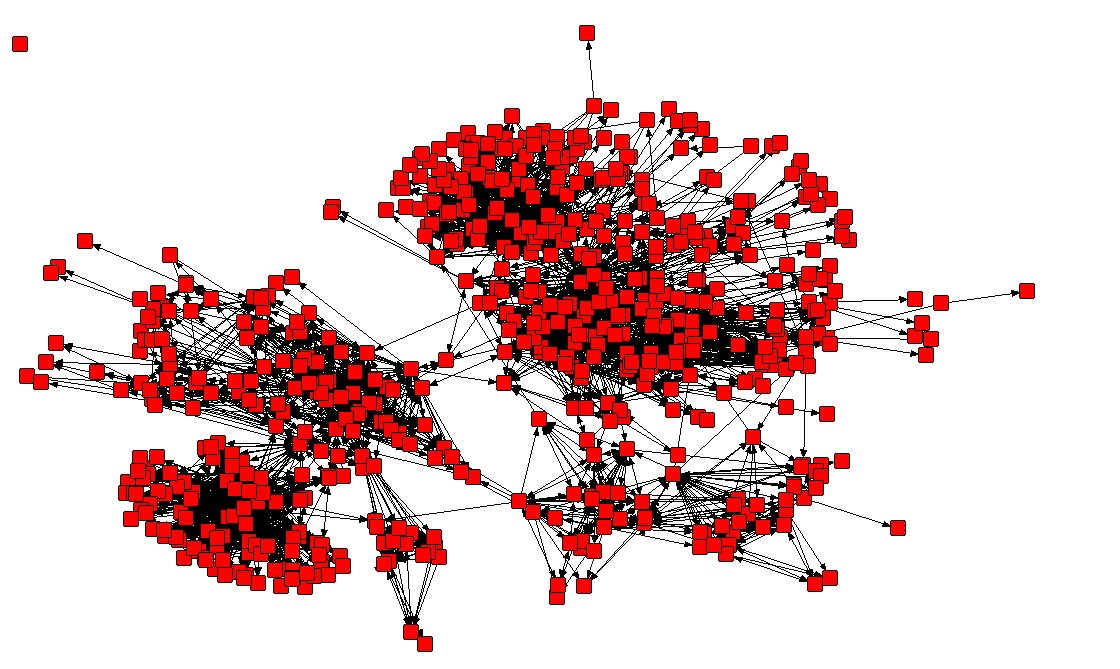
\includegraphics[width=\textwidth]{imgs/amigos-contatos.jpg}
\end{figure}

\section{mensuração textual}
\subsection{conceituação}
Na seção anterior investigamos as relações não-textuais, agora vamos nos deter
nas textuais. Primeiramente, intentamos com essa divisão alcançar uma
consequência prática: a integração de diversas interações numa só rede. A rede
que vamos construir é valorada, isto é, as conexões possuem um peso na forma de
um número real dentro de um intervalo. Ao contrário de redes binárias, as redes
valoradas proporcionam um indicativo da \textit{força} do laço entre os atores.

Dentro de uma teoria da atenção como capital social, devemos então nos voltar
para a afirmação de que laços por onde trafegam muito recursos são laços fortes
e o contrário também é verdade. Em cada interação na rede, como vimos, tem um
ator-agente que inicia a interação e um grupo de abrangência, que chamaremos de
atores-receptores, que é afetado por ela. Com esse modelo, podemos estimar que
os receptores cedem atenção para o agente e a recíproca também é verdadeira,
pois o agente escolheu interagir com este grupo e essa escolha já é um
indicativo de atenção cedida.

Idealmente, essa atenção poderia ser mensurada a partir do tempo empregado pelos
atores na interação, mas quase nunca essa informação está disponível. Por esta
razão, sugerimos a quantidade de palavras na interação textual como uma
estimativa para a quantidade de atenção trocada na interação. A sugestão advém
naturalmente do fato de que quanto maior o texto, mais tempo é empregado na sua
leitura, possivelmente mais recursos cognitivos também serão empregados para a
sua apreensão. Isso nem sempre é verdade para todos os textos, ou tipos de
textos, mas restringindo nosso escopo para comunidades virtuais de amigos e/ou
comunidades de prática, acreditamos ser esse um bom ponto de partida.

Outro cuidado necessário é na determinação se de fato a interação foi percebida
pelos receptores. Na maioria das vezes essa determinação é inviável, aumentando
a incerteza do modelo. Etretanto, um recurso simples que pode ser utilizado é
procurar por interações encadeadas, isto é, quando uma interação posterior é 
reação a outra anterior. Por exemplo, quando uma mensagem é respondida, um texto
é comentado, um conteúdo é recomendado, em todos esses casos podemos avaliar que
o agente que reagiu não só percebeu a interação do agente anterior, como se deu
o trabalho de responder. Em verdade, para interações que normalmente se
encadeiam como \textit{threads} de fórums ou listas de discussão, podemos
considerar a resposta como um sinal de atenção não só para com o participante
imediatamente anterior, mas para vários antes dele que de certa forma
influenciaram na resposta atual.

Assim, podemos construir uma rede onde os nós são os atores e os laços é o
somatório da atenção trocada pelos mesmos. Quanto mais textos de um ator $a$
lidos, respondidos, recomendados, avaliados por um ator $b$, maior será a força
da relação direcionada de $b$ para $a$. Quanto mais conteúdo um ator $a$ publica
para um determinado público, mais forte também será sua relação direcionada
com o mesmo. Tal rede, por tanto, integraria insumos de diversos tipos de
interação mensurados, desde que sejam de conteúdo textual.

No entanto, uma ultima consideração deve ser feita, a de que todos nós temos uma
quantidade limitada de atenção para ceder uns aos outros. Sendo assim, na
representação apresentada acima, a soma das forças dos laços para todo ator da
rede deve ser normalizada, de forma que atores que recebam interações de menos
agentes tenham laços mais fortes com eles do que receptores de grande quantidade
de agentes diferentes com os seus. Em termos gerais, quanto mais pessoas dividem
sua atenção, menos elas recebem proporcionalmente.

\subsection{formalização}
\label{sec:formalizacao}
Para a formalização dessa métrica, vamos usar um exemplo prático. Em um fórum
qualquer, vamos tomar um tópico para nosso exemplo. O fórum é o
\textbf{medianeiro}, os membros assinantes do fórum os \textbf{atores}. O tipo
de interação é \textbf{textual} quanto ao conteúdo, \textbf{comum} quanto a
abrangência e nossa análise será \textbf{ingênua}, isto é, não consideraremos a
intenção. Considere:
\begin{itemize}
  \item $G$ o conjunto de $n$ atores e $g_{1..n}$ uma sequência sobre $G$;
  \item $I$ o conjunto de $m$ tópicos do fórum e $i_{1..m}$ uma sequência sobre
  $I$;
  \item $A:I\to G$ tal que $A(i_k)$ seja o autor do tópico $i_k$, a função $A$
  não é inversível, dado que um ator pode ser autor de mais de um tópico, porém
  considere a função $A^{-1}:G\to \mathcal{P}(I)$ tal que $A^{-1}(g_h) = \{x \in
  I|A(x) = g_h\}$ representando o conjunto de tópicos escritos pelo ator;
  \item $R:I\to \mathcal{P}(G)$ tal que todo $x \in R(i_k)$ é um receptor de
  $i_k$, considere também o conjunto de tópicos recebidos por um ator como sendo
  $R^{-1}:G\to \mathcal{P}(I)$ tal que $R^{-1}(g_h) = \{x \in I|g_h\in R(x)\}$;
  \item $|i_k|$ como a quantidade de palavras de $i_k$; 
\end{itemize}

Definimos a atenção total cedida de $g_i$ para $g_j$, $p(i,j)$ como a soma de
suas atenções diretas, residuais e transitivas. A atenção direta é aquela
formada quando $g_i$ é receptor de $g_j$ e definimos como:

\begin{equation}
\label{def:atedireta}
p_{dir}(i,j) = \sum \alpha |k|\text{, para todo $k \in \{x \in I| A(x)=g_j
\wedge g_i \in R(x)\}$}
\end{equation}

A atenção residual é cedida quando $g_i$ é autor de algum tópico recebido por
$g_j$ e definimos como:

\begin{equation}
\label{def:ateresidual}
p_{res}(i,j) = \sum \beta |k|\text{, para todo $k \in \{x \in I| A(x)=g_i
\wedge g_j \in R(x)\}$}
\end{equation}

A atenção transitiva é aquela $g_j$ recebe de $g_i$ se ele foi autor de algum
tópico que $g_i$ respondeu. Para definirmos $p_tra$ devemos antes modelar o
encadeamento dos tópicos. Seja $T:I\to I\cup\{\emptyset\}$, se $i_h=T(i_k)$
então $i_k$ é uma resposta a $i_h$, se $i_k$ é a mensagem que iniciou o tópico
então $T(i_k)=\emptyset$. Agora faça $T^*:I\to\mathcal{P}(I)$:

\begin{equation}
\label{def:thread}
T^*(i_k) = \left\{ \begin{array}{l l} \emptyset &\quad\text{se
$T(i_k)=\emptyset$}\\ \{T(i_k)\} \cup T^*(T(i_k)) &\quad\text{em todo outro
caso}\end{array} \right.
\end{equation}

Daí temos que $T^*(i_k)$ é conjunto de todas as $m$ mensagens anteriores na
\textit{thread} de $i_k$ e podemos definir uma sequência $t^*_{kn}$, onde
$n=1..m$, sobre esse conjunto considerando a ordenação trivial: $a > b \iff a\in
T^*(b)$. Dessa forma $i_k$ é uma resposta a $t^*_{k1}$, que por sua vez responde
a $t^*_{k2}$ e assim sucessivamente até a mensagem inicial. Levando em
consideração a definição em \ref{def:thread}, definimos a atenção transitiva
como:

\begin{equation}
\label{def:atetransitiva}
\begin{array}{ l l }
p_{tra}(i,j) = \sum_k\sum_l
(1-\alpha)\gamma^l|t^*_{kl}| &\quad\text{para todo $k$ tal que $i_k \in \{x
\in I| A(x)=g_i\}$}\\&\quad\text{e todo $l$ tal que $A(t^*_{kl}) = g_j$}
\end{array}
\end{equation}

A partir das definições em \ref{def:atedireta}, \ref{def:ateresidual} e
\ref{def:atetransitiva} podemos calcular a atenção total entre $g_i$ e $g_j$
como:

\begin{equation}
\label{def:atetotal}
p(i,j) = E(g_i)\frac{p_{dir}(i,j) + p_{res}(i,j) + p_{tra}(i,j)}{\sum_{k|g_k \in
G}p_{dir}(i,k) + p_{res}(i,k) + p_{tra}(i,k)}
\end{equation}

Evidentemente, este é um modelo exploratório para a mensuração de redes a partir
de interações textuais sob um ponto de vista generalista. Nesse sentido há muito
espaço para aperfeiçoamento dentro do campo experimental. Para finalizar,
devemos fazer mais algumas considerações:
\begin{itemize}
  \item $p(i,j)$ tem sua soma normalizada devido ao limite de atenção
  natural de cada um;
  \item Porém, cada pessoa dedica quantidades diferentes de atenção total aos
  medianeiros analisados, de forma que seria simplório normalizar todos em 1.
  Por esta razão, cada ator tem a soma de suas atenções distribuídas na rede
  normalizada em um fator $E(g_i)$ que indica o seu grau de atividade na rede.
  Esse fator, \textit{a priori} será sempre relativo e caso o escolhamos como
  sendo a razão do total de atenção cedido pelo ator sobre a maior atenção
  medida, teremos uma normalização absoluta para toda a rede baseada no seu
  máximo. O que pode não ser a melhor escolha, pois idealmente a restrição de
  atenção deve servir para reduzir a variância das forças dos laços na rede;
  \item O parâmetro $\gamma$ representa a força da influência de mensagens
  antigas na $thread$ sobre um determinado ator em sua participação atual. Por
  esta razão $0 \leq \gamma \leq 1$, sendo que $\gamma=0$ anula toda a atenção
  transitiva e $\gamma=1$ considera todas as mensagens anteriores como sendo
  igualmente influentes na mensagem atual;
  \item O parâmetro $\beta$ representa a atenção recíproca do agente para os
  seus recptores, também varia de 0 a 1, sendo que $\beta=0$ anula a atenção
  residual da composição e $beta=1$ indica que o autor da mensagem cedeu
  individualmente a cada receptor tanto quanto este para com ele. Um valor
  interessante para $\beta$ é o inverso da quantidade de atores na abrangência
  da interação em contexto. Assim, o autor cede uma fração igual para cada
  receptor que é tão menor quanto maior for seu público;
  \item O parâmetro $\alpha$ representa o quão certos estamos de que a interação
  foi recebida integralmente pelo receptor. A sua escolha depende de diversos
  fatores da análise empregada sobre os medianeiros, pois que para cada caso
  poderemos (ou não) averiguar a atenção média cedida por um ator a uma
  interação que lhe chega qualquer. Se $\alpha=0$ indica que caso o receptor não
  tenha respondido à interação de alguma forma, ele não foi influenciado por
  ela. $\alpha=1$ retira qualquer valor do fato do ator ter respondido ou não
  determinada mensagem, igualando os dois casos. Em geral, mesmo que tenhamos o
  indicativo de que o receptor recebeu a interação, é interessante manter um
  valor de $\alpha$ diferente dos extremos para premiar a relação entre atores
  que se respondem.
\end{itemize}

[revisar esta seção considerando o efeito da powerlaw das trhead, de que
threads com muitas mensagens naturalmente atraem mais mensagens]

\begin{figure}[h!]
  \caption{A rede de atenção nos fóruns do A.M.I.G.O.S.}
  \centering
    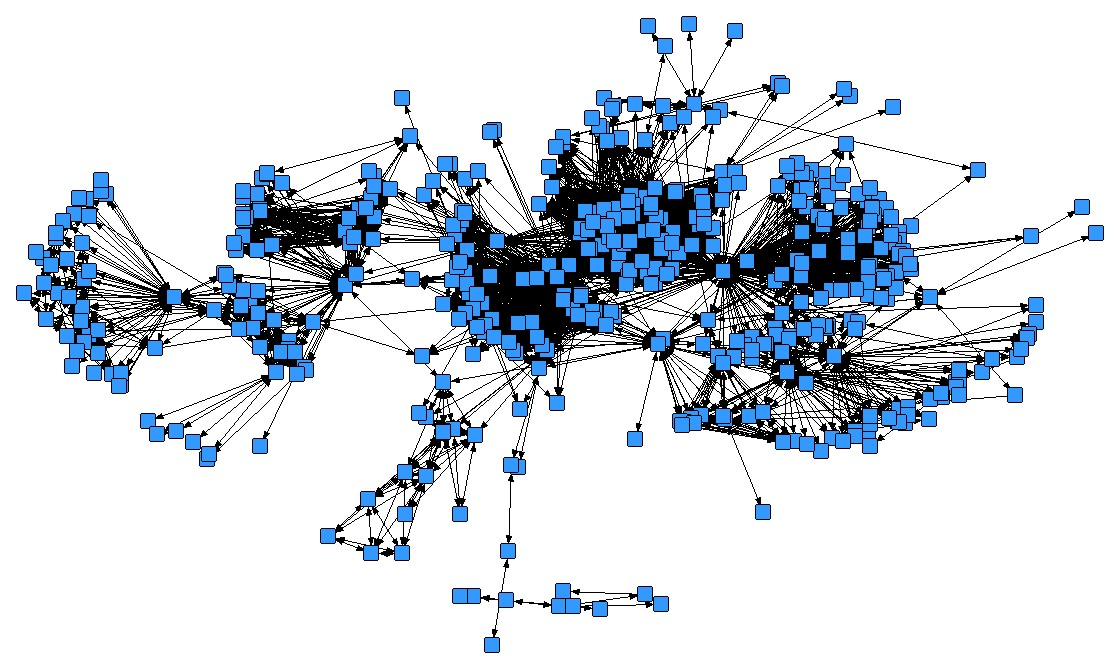
\includegraphics[width=\textwidth]{imgs/amigos-topicos.jpg}
\end{figure}

\begin{figure}[h!]
  \caption{A rede de atenção nas narrativas do A.M.I.G.O.S.}
  \centering
    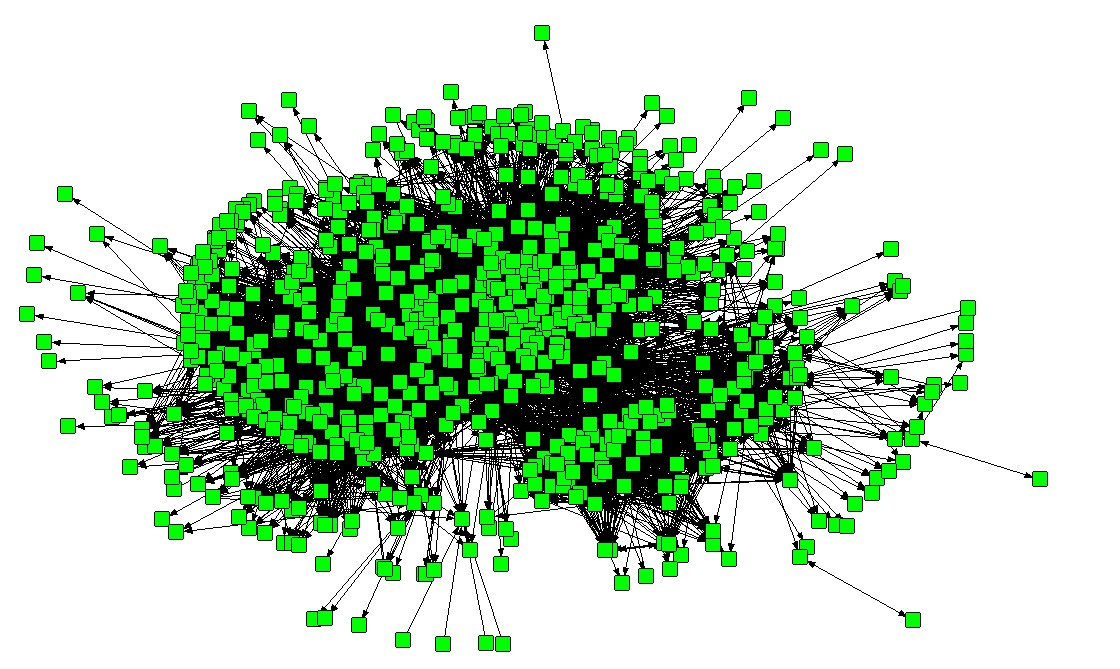
\includegraphics[width=\textwidth]{imgs/amigos-narrativas.jpg}
\end{figure}

\begin{figure}[h!]
  \caption{A rede de atenção total do A.M.I.G.O.S.}
  \centering
    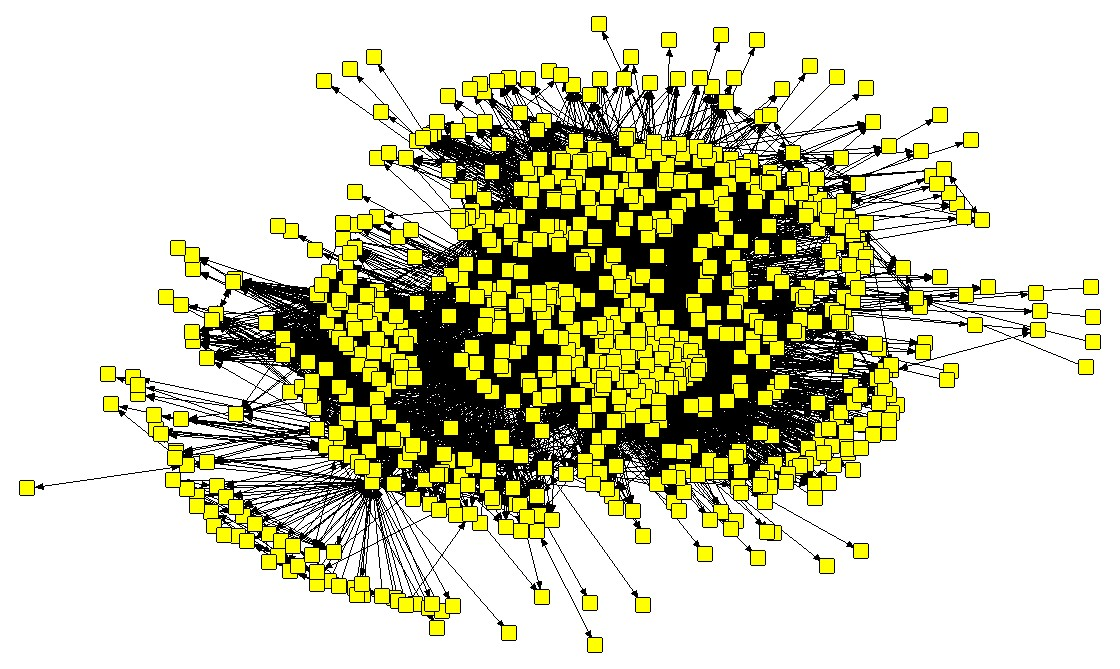
\includegraphics[width=\textwidth]{imgs/amigos-atencao.jpg}
\end{figure}

\begin{table}[htbp]
	\begin{boxedminipage}{\textwidth}
		Utilizamos a formalização descrita na seção \ref{sec:formalizacao} sobre a
		rede de teste do A.M.I.G.O.S. Os parâmetros foram:
		\begin{itemize}
		  \item $\alpha = 0.2$
		  \item $\beta = ^1/_\text{(quantidade da abrangência)}$
		  \item $\gamma = 0.5$
		\end{itemize}
		Foram consideradas os fórums e as narrativas (com seus comentários).
		Narrativas são similares aos \textit{posts} de \textit{blog} convencionais.
		Fizemos testes com várias possibilidades para $|i_k|$ pois a variância
		indicava muito ruído. Pode se ter como exemplo de ruído uma mensagem de
		fórum onde o autor copiou enorme lista com os nomes dos arquivos presentes na
		comunidade, nem o autor dedicou muito tempo ao copiar a lista, nem os outros
		membros devem ter dado muita atenção à lista inteira. Sendo assim, escolhemos
		um $|i_k|$ que desprezasse interações com quantidades de palavras muito
		destoantes. Fizemos $|i_k|=\tanh(0.5\lambda x)$ onde $x$ é a quantidade de
		fato de palavras e $\lambda=-\frac{\ln(10^{-4})}{\overline{x} + 5\sigma}$,
		$\overline{x}$ é a média e $\sigma$ é o desvio padrão, logo temos que pelo
		menos 95\% das interações encontram-se entre 0 e 0.9999.
		
		Foi coletado a rede usando apenas a interação por tópicos, depois por
		narrativas, depois as duas combinadas. A
		tabela~\ref{tab:comparacao_contato_atencao} apresenta uma comparação entre os
		quatro tipos de rede coletadas até agora.
		
% 		\large       % tamanho da fonte 
		\setlength{\arrayrulewidth}{2\arrayrulewidth}  % espessura da  linha
		\setlength{\belowcaptionskip}{10pt}  % espaço entre caption e tabela
		\caption{\it Comparação entre a rede de contatos e de atenção.}
		\centering   % tabela centralizada
		\begin{tabular}{| l | l | l | l | l |}
		\hline
		Métrica & Contatos & Fóruns & Narr. & Atenção \\ \hline
		Densidade & 0.0136 & 0.1861 & 0.05 & 0.05\\
		Reciprocidade & 0.5841 & 0.1120 & 0.83 & 0.79\\
		Coef. Cluster & 0.554 & 0.45 & 0.67 & 0.66\\
		Coef. Cluster Ponderada & 0.290 & 0.099 & 0.49 & 0.47\\
		Distância (geodésica) & 4.499 & 1.0340 & 2.54 & 2.63\\
		Coesão (Distância) & 0.183 & 0.983 & 0.43 & 0.41\\
		Largura (Distância) & 0.817 & 0.017 & 0.57 & 0.59\\
		Fitness (Núcleo/Periferia) & 0.257 & 0.0 & 0.44 & 0.44\\
		\hline
		\end{tabular}
		\label{tab:comparacao_contato_atencao}
		\flushleft
		\normalsize
		Nota-se uma maior adensamento da rede com encurtamento de caminhos nas redes
		de atenção. Porém enquanto a que foi formada a partir das interações nos
		fóruns tem menor coeficiente de \textit{clusterização} da rede com nenhum
		indicativo de padrão núcleo/periferia, a proveniente das narrativas tendência
		oposta. Pode-se dizer, que na rede do A.M.I.G.O.S. os fóruns descentralizam a
		distribuição da atenção, enquanto que as narrativas atuam em sentido
		contrário.
	\end{boxedminipage}
\end{table}

\section{critérios de escolha da representação}

Qual a rede ideal para o cálculo de proeminência? Não há resposta objetiva para
essa pergunta. Cada rede é uma representação de um fenômeno social que vai além
das ferramentas, mesmo sendo capaz de coletar e integrar todas as interações
digitais, as pessoas ainda vão ser capazes de tomar um café juntas e nossa visão
será apenas parcial. Sendo assim, é evidente que cada representação mensurada é
uma parte da informação e, portanto, capaz de descrever aspectos diferentes ou
não do fenômeno. São essas variações entre as representações de redes que
chamaremos de \textbf{critérios de escolha}.

Para enteder sua utilidade, um exemplo: imaginemos que ao final da análise
tenhamos duas ou mais representações da rede: uma textual e algumas não
textuais. Para cada uma encontramos valores diferentes de proeminência,
então qual usar? Colocando de outra forma, quanto de informação estarei perdendo
caso considere apenas uma delas? 

Esse é um problema bastante similar ao que estudiosos de aprendizagem de máquina
chamam de seleção de características (\textit{feature selection}) e que consiste
em decidir quais subconjunto de todas as variáveis possíveis que podem ser
utilizadas no treinamento da máquina são maximamente dependentes do resultado
esperado, ou seja, é maximamente relevante e minimamente redundante. No nosso
caso, porém, como afirmado acima, não há a rede \textbf{certa} e por isso a
relevância de todas elas são iguais. O que podemos procurar, portanto, é um
subconjunto com minimize a redundância. De acordo com o mais recente algoritmo
de mRMR (\textit{minimal-redundancy-maximal-relevance}) define-se a mínima
redundância como:

\begin{equation}
\label{def:min_redun}
\min R(S), R = \frac{1}{|S|^2}\sum_{x_i, x_j \in S}I(x_i, x_j)
\end{equation}

Onde $S$ é um subconjunto de características e $I(.)$ é a função de mútua
informação. Por definição, a função de mútua informação mede a correlação entre
duas variáveis aleatórias, porém, para o caso de redes sociais, o procedimento
comum é modelar cada par de ator como uma variável separada cujos valores
possíveis depende do tipo da rede. Se considerássemos cada rede como uma única
variável que representasse a chance de dois atores quaisquer estarem ligados,
então estaríamos nos limitando a uma correlação de suas densidades, o que de
forma nenhuma é interessante para nosso objetivo já que o cálculo de
proeminência varia consideravelmente a depender dos padrões das conexões,
mesmo em redes com densidade iguais.

Por esta razão, precisamos adaptar nossa função de mútua informação para
considerar as peculiaridades das redes sociais. Basicamente temos duas opções:
considerar a redundância das conexões ou calcular a proeminência para cada
rede e a partir daí determinar sua correlação. 

\subsection{Redundância das conexões}

Uma conexão é redundante quando pode ser encontrada em mais de uma rede. Mais do
que isso, duas redes são redundantes quando além de compartilhar conexões também
compartilham determinados padrões como triângulos e subgrupos. As duas
famílias de ferramentas para acessar essa similaridade estrutural mais
desenvolvidas na literatura são: gráficos aleatórios exponenciais e procedimento
de atribuição quadrática, respectivamente $p*$ (\textit{exponential random
graphs}) e \textit{QAP} (\textit{quadratic assignment procedure}).

\subsubsection{redes discretas e/ou esparsas}

O primeiro é mais apropriado para redes binárias ou com valores discretos.
Consiste em criar um modelo exponencial para a criação de grafos aleatórios a
partir de um conjunto de parâmetros relacionados a \textbf{configurações} de
interesse. Uma configuração pode ser desde a presença de uma conexão, até a
quantidade de k-triângulos e outros padrões mais complexos. Cada configuração
tem um parâmetro relacionado que pode ser negativo, indicando que a rede é tem
tendência inversa à presença daquela configuração, nula representando a
indiferença e positiva para uma tendência de mesmo modo. Assim sendo, cada
parâmetro pode ser visto como tendências da rede em relação a, por exemplo:
densidade, reciprocidade e transitividade da rede quando suas configurações
relativas são respectivamente a presença de conexões, a mutualidade das
relações e a presença de triângulos. 

Modelos exponenciais de gráficos aleatórios tem a seguinte forma geral:

\begin{equation}
\label{def:p_star_geral}
\Pr(\textbf{Y} = \textbf{y})
=\left(\frac{1}{k}\right)\exp\left\{\sum_A\eta_Ag_A(\textbf{y})\right\}
\end{equation}

Onde (i) o somatório é sobre todas as configurações procuradas em \textbf{y};
(ii) $\eta_A$ é o parâmetro relacionado à configuração $A$; (iii)
$g_A(\textbf{y})=1$ se a configuração é observada em \textbf{y}, ou 0 de outra
forma; (iv) $k$ é uma constante de normalização que garante que
(\ref{def:p_star_geral}) é uma distribuição de probabilidades. O vetor de
parâmetros $\eta$ é estimado para o grafo a ser modelado, procurando maximizar
a sua probabilidade, iterativamente a partir de simulações com o método Monte
Carlo (\textit{Markov chain Monte Carlo maximum likelihood estimation}).

Voltando ao problema de minimizar a redundância, podemos considerar o vetor
$\eta$ no cálculo de ``informação mútua'' entre as redes, no sentido de que
redes possuem a mesma informação se compartilham conexões e tendências similares
ao aparecimento de padrões estruturais. Derivamos $I_D$ para redes discretas:

\begin{equation}
\label{def:MI_discreto}
I_D(x, y) =\frac{\sum_{i,j = 1}^n x_{ij}y_{ij}}{\sum_{i,j = 1}^n
y_{ij}\sum_{i,j=1}^n x_{ij}} \rho(\eta_x, \eta_y)
\end{equation}

Onde (i) o numerador é a quantidade de conexões presentes em ambas $x$ e $y$;
(ii) o denominador da fração é a soma de todas as conexões de $x$ e todas de
$y$; e (iii) é a correlação linear entre os parâmetros $\eta$ estimados para $x$
e os estimados para $y$. Substituindo (\ref{def:MI_discreto}) em
(\ref{def:min_redun}) temos um modelo para o conjunto de redes com mínima
redundância.

\subsubsection{redes contínuas densas}

Para rede contínuas, um segundo método pode ser utilizado para calcular a
correlação diretamente. O procedimento de atribuição quadrática (\textit{QAP})
recomenda um modelo linear para a correlação das redes, assim, temos que:

\begin{equation}
\label{def:linear_model_qap}
Y = \alpha X + \epsilon
\end{equation}

A probabilidade de que a correlação encontrada não seja apenas coincidência é
acessada através da permuta das colunas da matriz seguindo algoritmo apropriado.
Não é nosso objetivo nos aprofundar na especifidades do teste, apenas é pertinente
considerarmos a  utilização da correlação linear como valor para a informação
mútua em \ref{def:min_redun} para redes de valores contínuos densos.

\subsection{Correlação de Proeminência}

O critério anterior busca relacionar as características da rede em busca de
informações redundante, porém também é interessante observar a relação que há
entre o produto final da análise das redes que são as medições de proeminência.
Para esse fim utilizaremos também a correlação linear de Pearson de forma que
duas redes podem estar positivamente relacionadas, aparentemente independentes
ou negativamente relacionadas. Um critério baseado na proeminência pode
correlacionar redes estruturalmente bastante diferentes, mas que resultam no
sobressaimento dos mesmos atores em termos de importância. Porém, se o objetivo
for minizar a redundância do ponto de vista da ordenação final dos atores por
grau de proeminência para a utilização em outros algoritmos como por exemplo,
escolha de subconjunto ótimo para marketing viral, então talvez este critério
seja o mais apropriado.

\begin{table}[htbp]
	\begin{boxedminipage}{\textwidth}
	No caso do A.M.I.G.O.S. só temos duas representações da rede, a primeira 
	proveniente da interação não textual ``contatos'', a segunda é a união de duas
	interações textuais: fóruns e narrativas. Sendo assim, só podemos avaliar o
	quão diferentes são as redes e por isso mesmo, o quanto de informação vamos
	perder escolhendo uma ou outra.
	
	Como a rede de contatos é binária a correlação linear fica prejudicada devido a
	limitação do modelo em relação a dados tão dicotômicos (0 ou 1), porém não
	temos uma implementação disponível de um algoritmo de estimativa no modelo $p*$
	para a nova configuração e executamos um teste de correlação QAP entre as duas
	redes. Verificamos que a rede de contatos e de atenção possuem um coeficiente
	de correlação positiva de 0.27, que quer dizer que a chance de encontrarmos um
	laço entre dois atores em ambas as redes é de 27\%. A chance de uma correlação
	nessa proporção acontecer entre as redes considerando uma combinação aleatória
	é menor que 0.001 e $R^2$ de apenas 0.07, parte devido à dicotomia dos dados.
	
	Também realizamos um teste de regressão para as duas métricas de proeminência
	escolhidas, o índice de poder de Bonacich e o de \textit{betweeness} de
	Freeman. Encontramos nenhuma correlação entre as redes para o primeiro,
	indicando que quanto a influência ambas as redes são bastante distintas. Já em
	termos de centralidade, pudemos verificar uma correlação positiva de 0.47, com
	$R^2=0.22$ e $p. < 0.0001$.
	
	Com essas medidas podemos avaliar melhor a perda de informação que teremos ao
	escolher apenas uma das redes. Não há necessidade de buscar um subconjunto de
	redes que minimize a redundância por que só temos 2 redes.
	
	\end{boxedminipage}
\end{table}

\subsection{Conclusão e trabalhos futuros}

Cada dia mais e mais interações entre pessoas ocorre em meio digital, essas
interações podem proporcionar a mensuração de diversas representações da rede
social que interliga estes indivíduos. O resultado deste processo pode alimentar
novas ações no campo do marketing, modelos sobre disseminação de idéias,
doenças e reconhecimento de especialistas. A seleção apropriada de medianeiros
para o recolhimento 

\title{PARTE II}

\section{outros problemas em relação às métricas de proeminência}

Voltando a questão da proeminência, mesmo que consigamos definir os medianeiros,
identificar os tipos de interação, mensurar a atenção investida e formalizar uma
rede direcionada e valorada, ainda assim teremos que a métrica pode não ser
significativa dependendo da parte da rede sobre o qual foi aplicada. Nota-se que
o que as métricas de proeminência fazem é verificar o envolvimento do nó com os
possíveis caminhos da rede como grafo. Nesse sentido, podemos dividir as
métricas em dois grandes grupos: as radiais que medem seu envolvimento nas
extremidades do caminho e as mediais que a fazem nos elos intermediários.

[relações intertextuais entre os atores para a formação de comunidades de
prática.]

Quando tudo o que temos é a rede para medirmos proeminência em atores de redes
sociais digitais precisamos de uma maneira de medir sua aplicabilidade.


% \center
\begin{tabular}{| l | l |}
\hline
Métrica & Valor \\ \hline
Densidade & 0.0136 \\
Reciprocidade & 0.5841 \\
Coef. Cluster & 0.554 \\
Coef. Cluster Ponderada & 0.290 \\
Distância (geodésica) & 4.499 \\
Coesão (Distância) & 0.183 \\
Largura (Distância) & 0.817 \\
Fitness (Núcleo/Periferia) & 0.257 \\
\hline
\end{tabular}

% \flushleft
A densidade, distância, coesão e largura nos diz que a rede é esparsa. O
coeficiente de clusterização mostra que apesar de que atores com poucos contatos
tem uma vizinhança relativamente interconectada, quanto maior a sua vizinhança,
menor a interconexão. Finalmente, o algoritmo de detecção de Núcleo/Periferia
encontrou baixa adequação. Todas essas métricas indicam que temos diversos
subgrupos dentro da rede e que ela está longe de se assemelhar a uma comunidade
de prática. Numa situação assim, [métricas mediais perdem força descritiva da
influência do ator na rede como um todo TODO: revisar isso aqui].


\end{document}
